\documentclass{beamer}
\usepackage[utf8]{inputenc}
\usepackage[english,russian]{babel}
\usepackage{hyperref}
\usepackage{xcolor}
\usepackage{graphicx}

\usetheme{Boadilla}
\usecolortheme{seahorse}
\setbeamercovered{transparent}% Allow for shaded (transparent) covered items

\AtBeginSection[]
{
  \begin{frame}
    \frametitle{Содержание}
    \tableofcontents[currentsection]
  \end{frame}
}

\begin{document}

\title[]{Многоагентные системы}
\author{Н.\,Д.~Кудасов}

\institute{
    % {\em Научный руководитель}:\\
    \vspace{2.0cm}
}
\date{Москва, 2013}

\begin{frame}
\addtocounter{framenumber}{-1}
\maketitle
\end{frame}

\section{Агенты}

\begin{frame}
  \frametitle{Что такое агент?}
  Агенты часто используются в области ИИ при разработке систем.
  Тем не менее, до сих пор не существует устоявшегося понятия.

  \begin{exampleblock}{}
    {\large ``Агент ~--- это инкапсулированная вычислительная система,
    помещенная в некоторую среду и способная автономно выполнять действия
    в этой среде для достижения поставленных целей.''}
    \vskip5mm
    \hspace*\fill{\small--- Wooldridge and Jennings}
  \end{exampleblock}

  % TODO: add distinct definition
\end{frame}

\begin{frame}
  \frametitle{Общее понятие}
  В самом общем случае агент обычно представляет нечто, обладающее
  следующими свойствами:

  \begin{itemize}
    \item<1-> {\it реакционность}: способность агента воспринимать окружающее и влиять на него;
    \item<2-> {\it целеустремленность}: агент должен действовать в заложенными в него целями;
    \item<3-> {\it социальная активность}: агент должен взаимодействовать с другими агентами и/или людьми;
    \item<4-> {\it автономность}: агент действует без непосредственного вмешательства человека и обладает
      определенным контролем на своими действиями и внутренним состоянием.
  \end{itemize}
\end{frame}

\begin{frame}
  \frametitle{Ментальность}
  Распространено использование ментальных характеристик:

  \begin{itemize}
    \item знания,
    \item убеждения,
    \item намерения,
    \item обязательства и т.п.
  \end{itemize}

  Иногда агенты наделяются {\it эмоциями}.
\end{frame}

\begin{frame}
  \frametitle{Прочие свойства}
  Часто также обсуждаются следующие свойства агентов:

  \begin{itemize}
    \item {\it мобильность}: способность агентов перемещаться (физически или в сети);
    \item {\it правдивость}: предположение, что агент не может намеренно фальсифицировать передаваемую информацию;
    \item {\it доброжелательность}: предположение, что цели агентов не конфликтуют и, следовательно, каждый агент
      стремиться выполнить то, о чём его просят;
    \item {\it рациональность}: предположение, что агент действует в соответствии со своими целями и не пытается
      противостоять себе (по крайней мере, насколько это позволяют его убеждения).
  \end{itemize}
\end{frame}

\begin{frame}
  \frametitle{Концепции агентов}
  Существует ряд формальных теорий, описывающих агентов:

  \begin{itemize}
    \item {\it логические системы}:
      цели и свойства агента описываются при помощи высказываний
      в различных логических системах;
    \item {\it системы намерений}:
      внутреннее состояние агента представляется системой
      мировоззрений (знания, убеждения, желания, намерения и т.п.);
    \item {\it модели коммуникаций}:
      взаимодействие между агентами происходит посредством специальных
      действий.
  \end{itemize}
\end{frame}

\section{Распределенная оптимизация}

\begin{frame}
  \frametitle{Сенсорная сеть}
  \begin{columns}[c]
    \column{.5\textwidth}
    \begin{itemize}
      \item каждый сенсор может выбрать 1 из 3 частот
      \item пересекающиеся сенсоры не должны иметь одну частоту
    \end{itemize}

    \column{.5\textwidth}
    \begin{figure}
       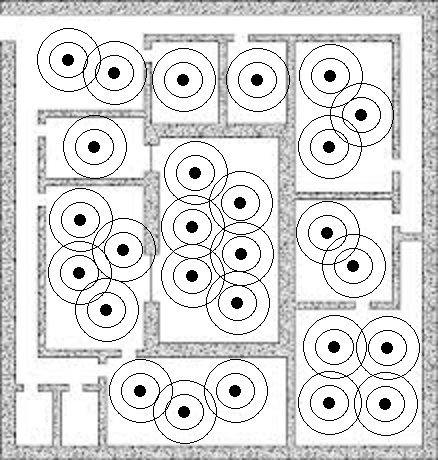
\includegraphics[width=5cm]{images/sensors.jpg}
    \end{figure}
  \end{columns}
\end{frame}

\begin{frame}
  \frametitle{Раскраска графа}
  \begin{columns}[c]
    \column{.5\textwidth}
    \begin{itemize}
      \item каждая вершина может быть раскрашена в один из трех цветов
      \item смежные вершины должны быть раскрашены в разные цвета
    \end{itemize}

    \column{.5\textwidth}
    \begin{figure}
       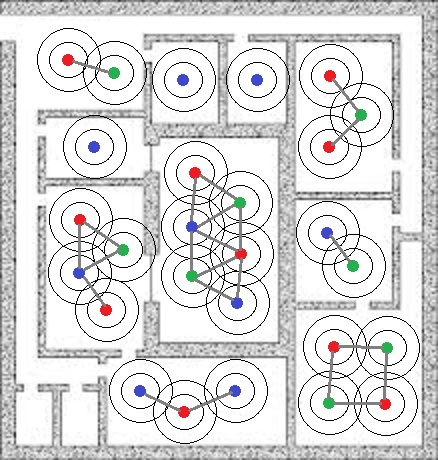
\includegraphics[width=5cm]{images/graph-coloring.jpg}
    \end{figure}
  \end{columns}
\end{frame}

\begin{frame}
  \frametitle{Задачи с ограничениями}
  Распределенная задача \alt<2>{\alert{оптимизации}}{с ограничениями}:
  \begin{itemize}
    \item множество переменных (сенсор, вершина);
    \item множества возможных значений для каждой переменной (частота, цвет);
    \item множество ограничений (перекающиеся сенсоры, смежные вершины);
    \item распределение переменных по агентам (обычно одна переменная на агента);
    \item<2-| alert@2> функция веса для каждого нарушенного ограничения;
    \item необходимо \alt<2>{\alert{минимизировать сумму весов нарушенных ограничений}}
      {назначить каждой переменной значение, чтобы ограничения были выполнены}.
  \end{itemize}
  \visible<3->{\alert{Задачи с ограничениями в общем случае NP-полные!}}
\end{frame}

\begin{frame}
  \frametitle{Распределенные алгоритмы}
  Подходы к решению:

  \begin{itemize}
    \item адаптация классических решений (не распределенных);
    \item адаптация алгоритмов локального поиска;
    \item кооперативные подходы.
  \end{itemize}
\end{frame}

\begin{frame}
  \frametitle{Асинхронный перебор (ABT)}
  Каждый агент отвечает за одну переменную и предлагает другим агентам принять значение,
  которое он выбрал.
  \begin{itemize}
    \item ABT ~--- полный алгоритм;
    \item глобальное упорядочивание агентов;
    \item нет процедуры останова (но она легко добавляется);
    \item хорошо масштабируется.
  \end{itemize}

  Расширения:
  \begin{itemize}
    \item изменение порядка при конфликтах (AWCS);
    \item решение задачи оптимизации (ADOPT, APO);
    \item динамическое добавление агентов (DynAPO).
  \end{itemize}
\end{frame}

\begin{frame}
  \frametitle{Распределенный локальный поиск}
  Алгоритмы распределенного поиска исследуют возможные изменения состояния:
  \begin{itemize}
    \item всегда стремятся улучшить состояние (уменьшить количество конфликтов);
    \item естественным образом поддерживают динамику (добавление ограничений, агентов);
    \item эффективны по времени;
    \item не полны и требуют настройки параметров.
  \end{itemize}

  Известные алгоритмы:
  \begin{itemize}
    \item Tabu search;
    \item Simulated annealing;
    \item Iterative Breakout method.
  \end{itemize}
\end{frame}

\begin{frame}
  \frametitle{Алгоритмы популяций}
  Популяция ~--- это набор индивидуальных агентов.
  \begin{itemize}
    \item агент знает целиком исходную задачу (и может решить сам);
    \item агенты координируются для нахождения решения.
  \end{itemize}

  Известные алгоритмы:
  \begin{itemize}
    \item эволюционные и генетические алгоритмы;
    \item Particle Swarm Optimization (PSO);
    \item Ant Colony Optimization (ACO).
  \end{itemize}
\end{frame}

\begin{frame}{}
\addtocounter{framenumber}{-1}
\begin{center}
\LARGE{Спасибо за внимание!}
\end{center}
\end{frame}

\end{document}

